% !TeX spellcheck = en_US


\chapter{Related Works}


\section{Whisker-Inspired Tactile Sensors}
Several structural designs have been proposed for whisker sensors.
They mainly differ in their transduction principle: how the normal force of contact is transferred to the sensor base.
The most common designs use passive, flexible cantilever whiskers integrated with strain gauges or piezoresistive elements to measure deflections.
Capacitive and optical variants also exist but are less widely used.
Additionally, magnetically transduced whiskers, although less common in industry, offer a low-cost and easily manufacturable alternative~\cite{8968518}.

\subsection{Magnetically Transduced Whisker Sensors}
Although magnetically transduced whisker sensors have yet to be widely adopted, they provide high precision and sensitivity, making them suitable candidates for tactile sensing.
Kim et al.~\cite{8968518} developed a magnetically transduced whisker sensor using a small permanent magnet attached to a flexible, cantilevered whisker.
Figure~\ref{fig:kim-whisker} illustrates this sensor design.
Its operating principle is straightforward: when the whisker contacts an object, deflection shifts the magnet embedded in a compliant, spring-like suspension relative to a magnetic sensor.
The magnetic field strength is therefore proportional to the moment applied at the whisker base.
Calibration is performed by measuring sensor output at various deflection angles and fitting the data using Gaussian process regression.
One advantage is easy waterproofing, as the whisker does not directly contact the sensor.
A limitation, however, is the rigidity of the whisker, complicating surface tracking.

Dang et al.~\cite{dang2025whisker} introduced a magnetically transduced whisker sensor employing a flexible nitinol wire as the whisker.
They proposed a suspension device comprising three integrated, flexible spiral arms.
Their sensor structure, shown in Figure~\ref{fig:dang-whisker}, resembles Kim et al.'s design.
They assume tip contact and model the tip position based on the whisker's deflection profile, parameterized using the one-dimensional measurement from a Hall sensor along the respective axis.
A limitation of their approach is the indistinguishability of tip and tangential whisker contacts, as both produce identical deflection profiles at the whisker base.

\begin{figure}[htb]
    \centering
    \begin{subfigure}{0.48\textwidth}
        \centering
        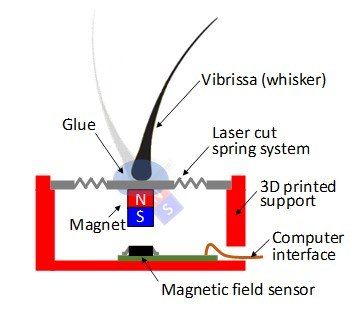
\includegraphics[width=\textwidth]{figures/kim-velez-whisker}
        \caption{Magnetically transduced whisker sensing mechanism schematic by Kim et al.~\cite{8968518}.}
        \label{fig:kim-whisker}
    \end{subfigure}\hfill
    \begin{subfigure}{0.48\textwidth}
        \centering
        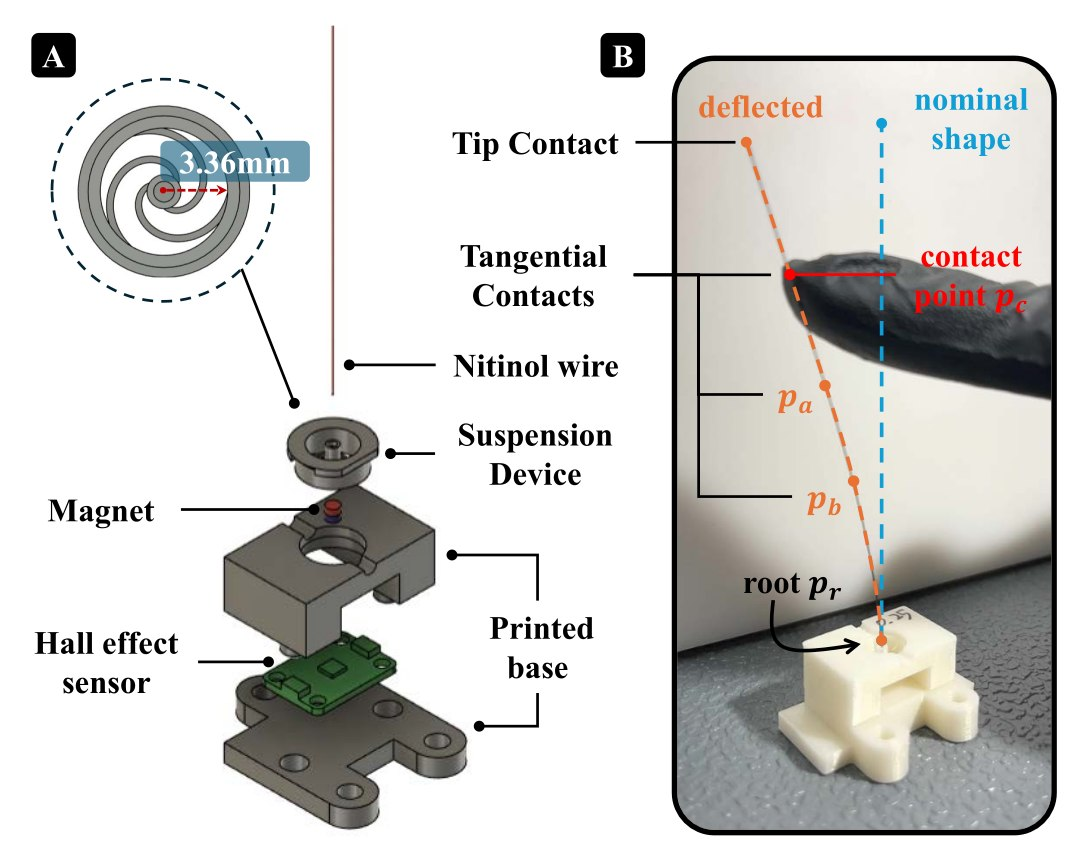
\includegraphics[width=\textwidth]{figures/dang-whisker}
        \caption{Structure of whisker-inspired tactile sensor by Dang et al.~\cite{dang2025whisker}.}
        \label{fig:dang-whisker}
    \end{subfigure}
    \caption{Side-by-side comparison of whisker sensor designs.}
\end{figure}

\subsection{Piezoresistive Whisker Sensors}
Piezoresistive whisker sensors are the most common type, notably applied in marine robotics to detect water flow and pressure variations.

Guo et al.~\cite{GUO2024114875} developed a piezoelectric wavy whisker sensor (PWWS) inspired by seal whiskers.
The sensor consists of a flexible, waterproof PDMS body and a thin sensing layer made of PVDF.
PDMS, a rubber-like material, protects the sensor from water, while PVDF is a polymer generating a small electrical voltage when bent or pressed.
When water flows around an object, vortices form, pushing against the whisker, bending the PVDF layer, and producing a voltage as depicted in Figure~\ref{fig:piezoelectric-whisker}.
The generated voltage correlates with water flow parameters, enabling tracking of underwater disturbances.

\begin{figure}[htb]
    \centering
    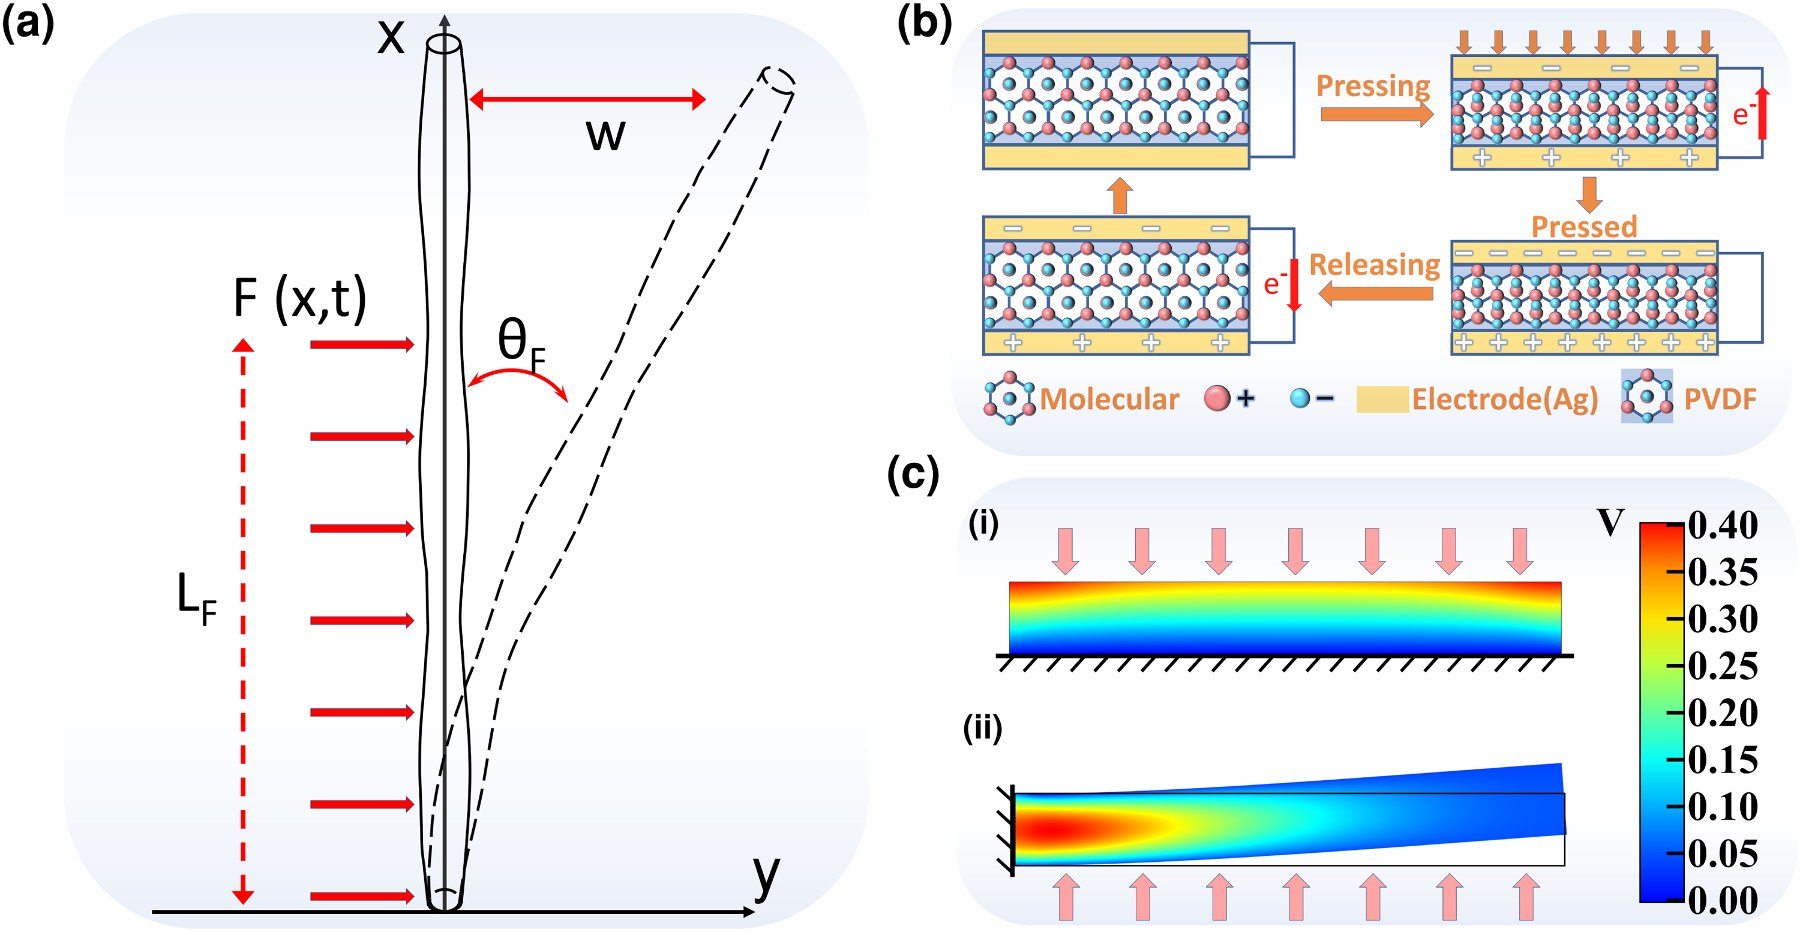
\includegraphics[width=\textwidth]{figures/piezoelectric-whisker}
    \caption{Operating principles of the PWWS by Guo et al.~\cite{GUO2024114875}. (a) Schematic of whisker deflection under force. (b) Cycle of electrical signals generated by the piezoelectric sensing unit. (c) Simulation of piezoelectric voltage within PVDF material under various constraints when subjected to external forces.}
    \label{fig:piezoelectric-whisker}
\end{figure}

\subsection{MEMS Whisker Sensors}
Wei et al.~\cite{9114501} developed a MEMS-based biomimetic whisker sensor replicating the tactile sensing mechanism of rats.
The sensor is integrated onto a small silicon chip (6.8\,mm square) containing four identical sensing units.
Each unit mimics the follicle arrangement of a rat's whisker, featuring a flexible whisker shaft attached to a central hub and four beams.
Piezoresistors implanted on these beams form a Wheatstone bridge.
Whisker bending from contact changes the resistance, producing an electrical signal.
The sensor fabrication uses standard MEMS processes, and the resulting structure is shown in Figure~\ref{fig:mems-whisker}.
Production begins with an SOI wafer, followed by ion implantation, insulating and metal layer deposition, and beam etching.
Experiments indicate the sensor reliably measures contact distances (30--40\,mm), recognizes object shapes (round, flat, beveled), and differentiates textures.
Thus, this whisker sensor has significant potential for integration into robotic systems requiring tactile sensing.

\begin{figure}[htb]
    \centering
    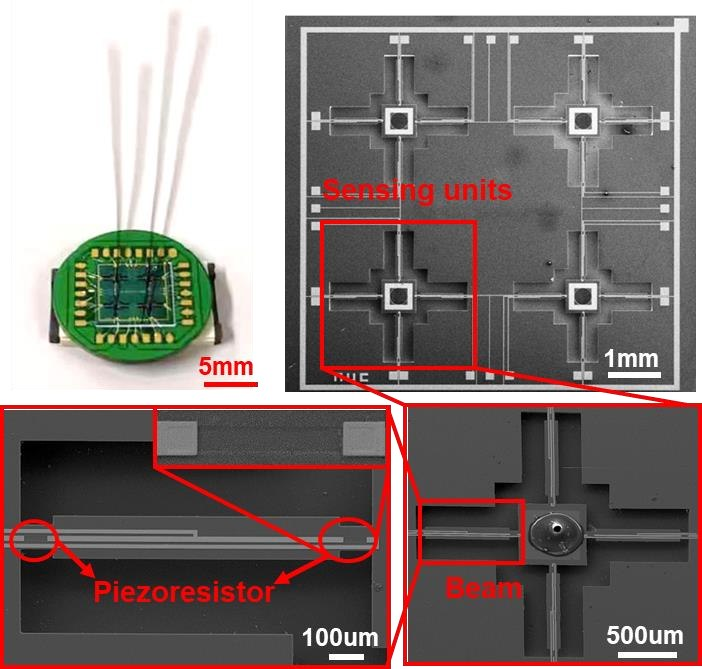
\includegraphics[height=0.4\textheight]{figures/mems-whisker}
    \caption{SEM image of the MEMS-based biomimetic whisker sensor by Wei et al.~\cite{9114501}.}
    \label{fig:mems-whisker}
\end{figure}


\section{Active Tactile Exploration}

This thesis is largely based on the work of Dang et al.~\cite{dang2025whisker}, who, besides the whisker sensor, also developed a control system for active tactile exploration.
They
\subsection{Previous Work}

